\documentclass[a4paper, table, 11pt]{article}

%----------------------------------
% Graphics, figures, colour, and tables
%----------------------------------
\usepackage{graphicx}                  % For including images
\usepackage{float}                     % For precise figure/table placement using [H]
\usepackage{longtable}
\usepackage{caption}                   % Customisation of figure/table captions
\usepackage{xcolor}

\usepackage{tabularx}                  % Tables with flexible-width columns
\usepackage{tabu}                      % Extended table capabilities
\usepackage{booktabs}                  % Improved horizontal rules in tables
\usepackage[numbers]{natbib} % Enables numbered citations

%----------------------------------
%Custom commands (for development notes)
%----------------------------------
\newcommand{\todo}[1]{\textcolor{red}{\bf [[TODO: #1]]}}
\newcommand{\instructions}[1]{\textcolor{blue}{\textbf{[[Remove before submitting:} #1]]}}


\newcommand{\update}[1]{\textcolor{blue}{\textbf{[[Update before submitting:} #1]]}} %Instructions to be removed before submitting


%----------------------------------
% Document layout and structure
%----------------------------------
\usepackage[utf8]{inputenc}            % Support for UTF-8 encoded input
\setlength{\parskip}{1em}              % Adds vertical space between paragraphs
\usepackage[margin=2.5cm]{geometry}    % Set custom page margins
\usepackage{titlesec}                  % Custom formatting for section headings
\usepackage{titletoc}                  % Custom table of contents formatting
\usepackage{appendix}                  % Support for appendices

% Automatically include bibliography and appendix in TOC, but not TOC itself
\usepackage[nottoc,numbib]{tocbibind}

\usepackage{fancyhdr}                  % Allows customization of headers and footers

\usepackage{hyperref}                  % Enables clickable references and links
\hypersetup{
    colorlinks=true,                   % Use colored text for links (instead of boxes)
    linkcolor=blue,                    % Color for internal links
    citecolor=blue,                    % Color for citation links
    urlcolor=blue                      % Color for URL links
}
\urlstyle{same}                        % Keep URLs in the same font as the surrounding text


%----------------------------------
%TikZ graphics for cover page
%----------------------------------
\usepackage{tikz}                      % Drawing diagrams and layout elements
\usetikzlibrary{positioning, calc}     % Extra TikZ libraries for positioning and calculations

% Define coordinate extraction command used on the title page
\makeatletter
\newcommand{\gettikzxy}[3]{%
  \tikz@scan@one@point\pgfutil@firstofone#1\relax
  \edef#2{\the\pgf@x}%
  \edef#3{\the\pgf@y}%
}
\makeatother

%----------------------------------
%Acknowledgements
%----------------------------------
\newenvironment{acks}{
  \section*{Acknowledgments}
  \addcontentsline{toc}{section}{Acknowledgments}
}{}

\newcommand\reporttitle{Work Integrated Learning Project: Written Report}
\newcommand\reportsubtitle{COSC2669\\Case Studies in Data Science\\2026}
\newcommand\groupnumber{\textbf{WIL Project 9}}
\newcommand\groupmentor{Mentor: Syeda Khan}
\newcommand\logopath{img/rmit-university-logo-png-transparent.png}
\newcommand\placeanddate{School of Computing Technologies \\ RMIT University \\ 2026}
\newcommand{\authorlist}{}
\newcommand{\addauthor}[2]{\gappto\authorlist{#1 & #2 \\}}
\pagestyle{fancy}
\lhead{\groupnumber}
\rhead{FinTrace: Written Report}
\setlength{\headheight}{14pt}
\setlength{\emergencystretch}{2em}
\renewcommand{\footrulewidth}{0.4pt}
\cfoot{Page \thepage}
\begin{document}
\addauthor{Ayushi Negi}{s4196173}
\addauthor{Janhavi Maheshwar Ghate}{s4188725}
\addauthor{Shriram Varadarajan}{s4162697}
\addauthor{Guruprasad Simimath}{s4188084}
\addauthor{Yash Keswani}{s4177991}
\addauthor{Hashini Santhanakrishnan}{s4163868}
\begin{titlepage}
\centering
\begin{tikzpicture}
    \node[inner sep=0pt] (logo) at (0,0)
        {\includegraphics[width=.3\textwidth]{\logopath}};
    \node[text width=0.5\textwidth, right=of logo](title){\sffamily\huge\reporttitle};
    \node[text width=0.5\textwidth, yshift=0.75cm, below=of title](subtitle){\sffamily\Large\reportsubtitle};
    \gettikzxy{(subtitle.south)}{\subtitlex}{\subtitley}
    \gettikzxy{(title.north)}{\titlex}{\titley}
    \draw[line width=1mm]($(logo.east)!0.5!(title.west)$) +(0,\subtitley) -- +(0,\titley);
\end{tikzpicture}
\vspace*{\stretch{1}}
{\sffamily\Large\textbf{FinTrace: Making Sense of Bank Reports}\par}
\vspace{0.6cm}
{\sffamily\Large\groupnumber\par}
\vspace{0.5cm}
{\sffamily\large\groupmentor\par}
\vspace{1.5cm}
\begin{table}[H]
    \centering\sffamily\large
    \begin{tabu} to 0.8\linewidth {cc}
        \textbf{Full Name} & \textbf{Student ID} \\
        \hline
        \authorlist
    \end{tabu}
\end{table}
\vfill
{\small\href{https://www.overleaf.com/project/6a825099db573616c529838b}{Shared Overleaf project and version history}\par}
\vspace{0.5cm}
{\sffamily\Large\placeanddate}
\end{titlepage}
\newpage
\pagenumbering{roman}
\section*{Executive Summary}
\addcontentsline{toc}{section}{Executive Summary}
Financial analysts reviewing bank results need to understand not only the reported figures but also what those figures represent. Similar measures can differ in accounting basis, reporting period or operational scope, making it important to check the original evidence before using an answer in a financial briefing.

FinTrace is a retrieval augmented generation (RAG) prototype that helps analysts explore six official Commonwealth Bank of Australia and National Australia Bank reports covering FY2024 and FY2025. Users can find financial figures, compare results across years within a bank, understand financial terms and explore management's explanations. Answers include relevant financial context and references to the original report pages. Python performs supported calculations using checked source values, while a local language model helps select relevant passages and explain financial terms.

Development followed an iterative testing process covering document extraction, chunking, retrieval and answer production. Testing revealed problems including figures separated from their labels, incorrect associations between financial measures and incomplete answers. These findings guided improvements to evidence handling and response coverage. Investigating one apparent system error also uncovered a mistake in the expected answer, demonstrating the importance of checking evaluation references against the original reports.

The resulting prototype brings financial answers, supporting evidence and calculation workings into one interface. It supports an analyst's review while making evidence limitations visible. Some explanations remain incomplete and response times vary, providing clear priorities for further development. FinTrace demonstrates how testing throughout the RAG pipeline can produce a more useful and accountable tool for exploring financial reports.

\newpage
\addcontentsline{toc}{section}{Contents}
\tableofcontents\thispagestyle{empty}
\newpage
\listoffigures\thispagestyle{empty}
\vspace{1.2em}
\listoftables\thispagestyle{empty}
\newpage
\pagenumbering{arabic}
% Report section owner: Ayushi Negi.
% AI-assisted working draft: review the wording, sources and scope with the team before submission.
\section{Problem Definition}
\label{sec:Problem Definition}

\subsection{Stakeholder and motivation}
Financial analysts reviewing Australian bank results need to locate, interpret and compare information spread across lengthy reports. Finding a figure is only part of the task. Before using it in a briefing, an analyst needs to understand what it measures, which reporting period it covers and whether it can be compared with another result. This context may be distributed across results releases, management commentary and accounting notes.

Commonwealth Bank of Australia's (CBA) FY2025 Profit Announcement illustrates the problem. It reports four profit figures: cash and statutory profit, each for continuing operations and for the total including discontinued operations. For example, continuing cash profit is AUD~10,252 million, while total statutory profit is AUD~10,116 million. Both are valid, but they represent different results. An answer that omits these distinctions can be misleading even when its number appears in the report~\cite{fintraceCBA2025}.

FinTrace addresses this problem of finding financial information without losing its meaning. It supports an analyst's review by making the answer and its evidence available together. The analyst remains responsible for interpreting the information before using it in a briefing or financial review.

\subsection{Aim and project questions}
The project aims to develop and evaluate a RAG assistant that helps financial analysts find and understand reported information. Users can ask questions, compare supported results across years, look up financial terms and explore management's explanations. Answers provide relevant context, source pages and calculation workings where applicable.

The project investigates four questions:
\begin{enumerate}
\item Can FinTrace find the requested information while preserving its company, reporting period, unit, financial meaning and the parts of the business it covers?
\item Can it compare figures measured on the same basis across two financial years within a bank and show how the change was calculated?
\item Can it explain financial terms and reported changes using relevant evidence without presenting an unsupported interpretation as a reported fact?
\item Can it recognise when the available evidence is insufficient and communicate that limitation without inventing an answer or substituting another measure?
\end{enumerate}
Evaluation considers correctness, completeness, supporting citations, calculations and the handling of unanswered questions. Declining a request can be appropriate when evidence is insufficient, but declining a question the system should answer is a limitation. Response time is assessed separately.

\subsection{Scope and changes since Milestone 1}
The prototype covers six official reports from CBA and National Australia Bank (NAB) for the financial years FY2024 and FY2025. Milestone~1 proposed an assistant for corporate reports with separate Ask and Verify modes, including claim verdicts. We refined this into one question interface focused on banking. Selecting one sector and two years made it feasible to understand the terminology, check reference answers and evaluate historical comparisons~\cite{fintraceMilestone2026,fintraceSources2026}.

Initial testing focused on 13 core financial measures and selected tables. However, treating that list as the boundary for every question excluded useful definitions and management commentary. We therefore expanded text search across the full reports and added checks for further NAB financial tables. General profit and earnings per share questions also retain the available labelled alternatives. Calculations remain restricted to values checked against their sources~\cite{fintraceCoverage2026,fintraceBroad2026}.

Supported comparisons are between years within the same bank. Comparisons between banks remain outside the prototype's scope and would require additional checks of reporting periods and definitions. CBA and NAB have different financial year ends. Live prices, future profit predictions, private account information and personalised investment advice are also excluded. The deliverable is a local research prototype that supports evidence checking rather than replacing professional financial judgement.

% AI-assisted overview and figure integration, 25 October 2026.
% Methodology coordinator: Ayushi Negi. Review with the assigned section reviewers.
\section{Methodology}
\label{sec:Methodology}

The final implementation is available in the group's \href{https://github.com/AyushiNegi20/COSC2669-WIL-PROJECT}{WIL project repository}. FinTrace uses separate processes for preparing documents, retrieving evidence and producing answers. Figure~\ref{fig:fintrace_architecture} shows how structured financial tables and prose from the full reports reach the appropriate answer process. Both retain references to their sources. Evaluation questions and expected answers are kept outside the evidence used by the application.

\begin{figure}[!htbp]
\centering
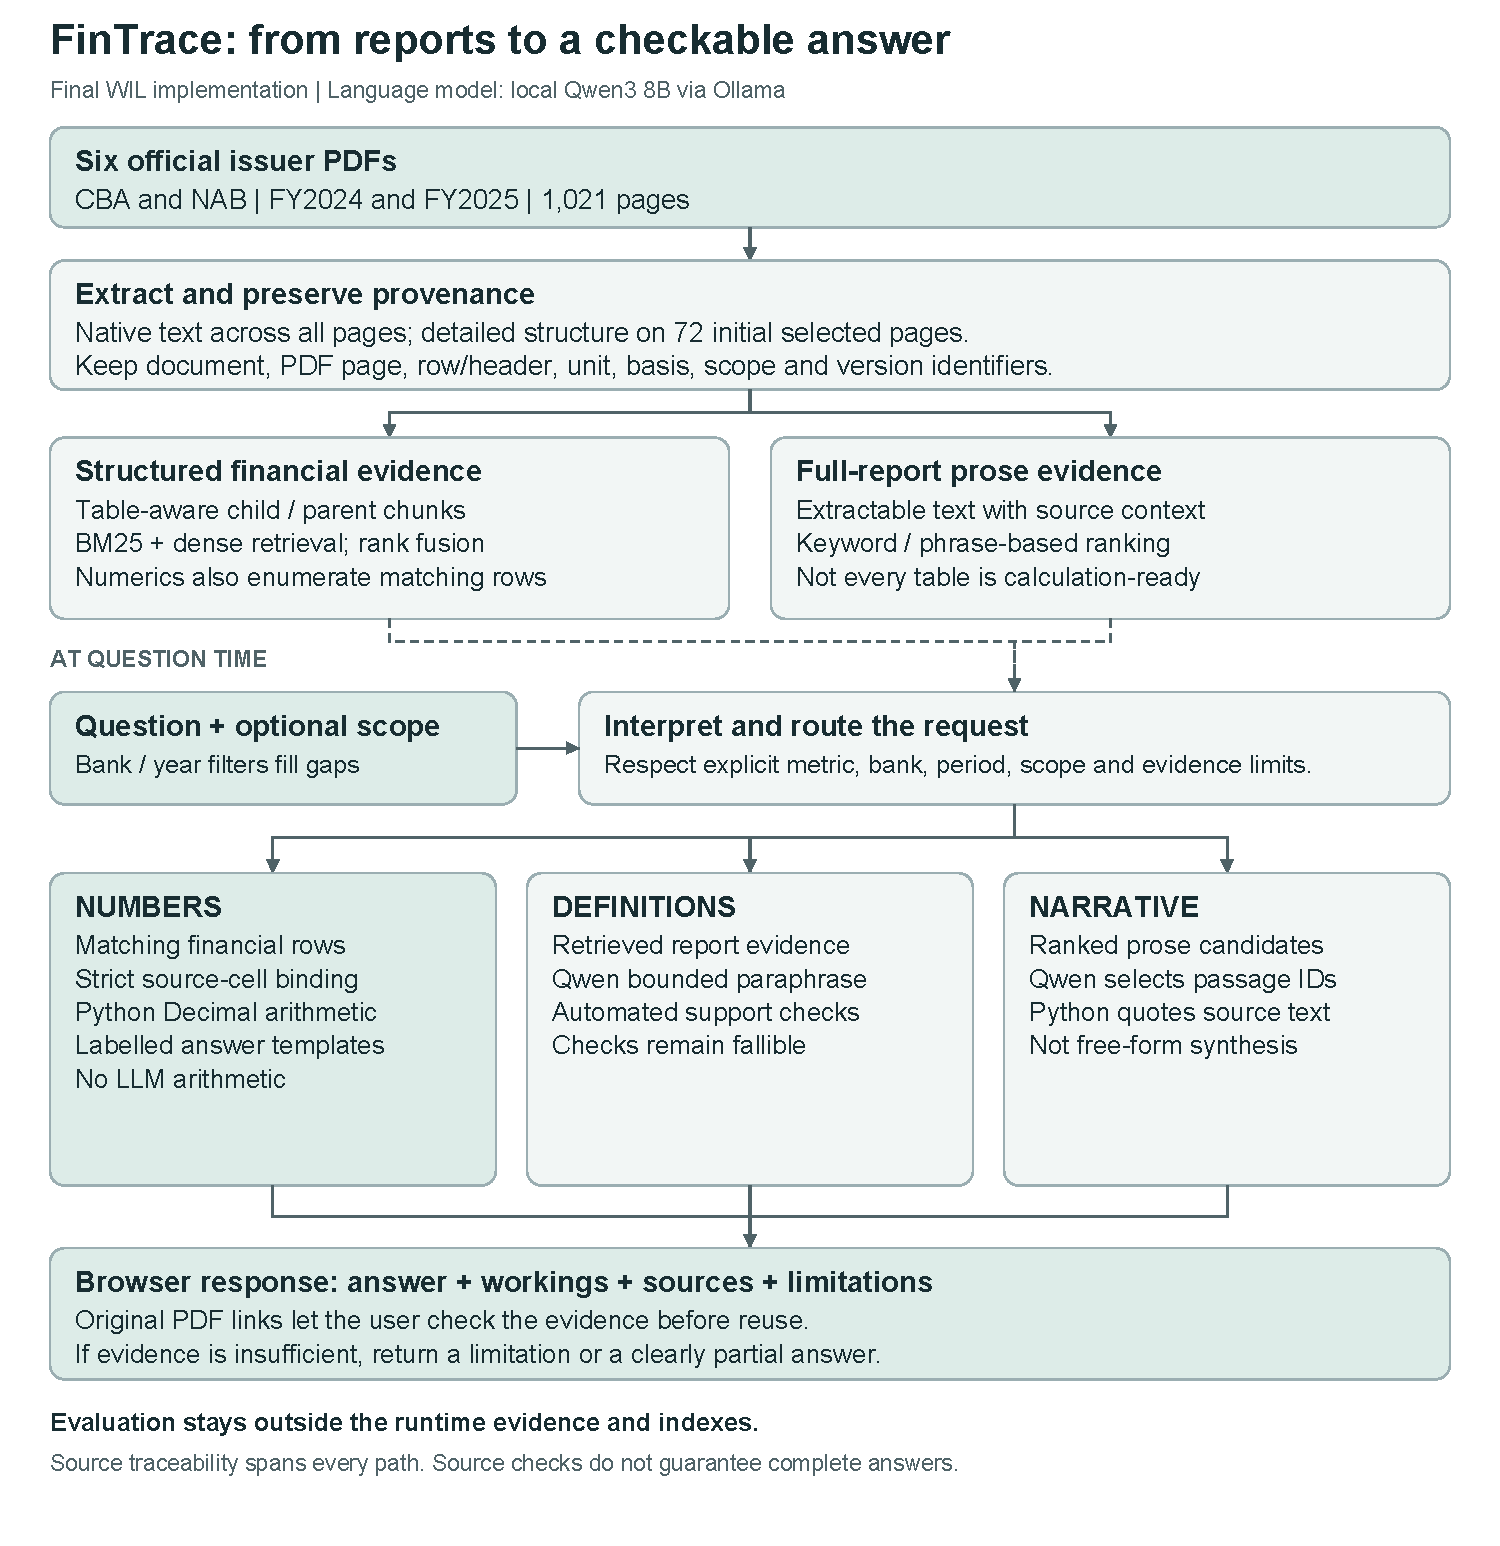
\includegraphics[width=0.98\linewidth,height=0.78\textheight,keepaspectratio]{fintrace_architecture.pdf}
\caption[FinTrace architecture]{Architecture of the final FinTrace implementation. Technical version details are recorded in Appendix~\ref{app:implementation_versions}. Structured evidence combines keyword and semantic retrieval, while prose uses keyword search followed by local model passage selection. Supported numerical answers link values to source cells and use Python for arithmetic. Qwen3 8B through Ollama supports passage selection and definitions. Dashed connections show evidence supplied to the relevant answer process~\cite{fintraceRuntime2026}.}
\label{fig:fintrace_architecture}
\end{figure}

% AI-assisted shared draft prepared at Ayushi's request on 25 October 2026.
% Assigned reviewer: Yash Keswani. Verify sources before approval; this is not personal authorship evidence.
\subsection{Data Sources and Scope}
\label{subsec:data_sources}

The knowledge base contains six official issuer reports for Commonwealth Bank of Australia (CBA) and National Australia Bank (NAB), covering FY2024 and FY2025. These comprise two CBA Profit Announcements, two NAB full-year results releases and two NAB Annual Reports, totalling 1,021 PDF pages. The source manifest records each document's title, issuer URL, reporting period and checksum~\cite{fintraceSources2026}. Results releases concentrate performance tables and management commentary~\cite{fintraceCBA2025,nabResults2025}; the NAB annual reports provide supporting accounting notes and reconciliations~\cite{nabAnnual2025}.

Banking provided a manageable domain with repeated measures and public evidence against which answers could be checked. Two years allow historical comparisons within a bank. However, CBA's year ends on 30 June and NAB's on 30 September: an identical financial-year label does not establish identical reporting periods. The prototype declines explicit cross-bank comparisons rather than treating them as directly comparable.

All reports received native-text extraction. An initial selection of 72 pages supported detailed structured extraction and checking; later indexing expanded searchable prose across the full reports. These are different coverage levels. Searchable text does not make every chart or table reliable enough for calculations. The original thirteen measure families defined a starting numerical scope, not a claim that other financial information was absent.

% Report section owner: Ayushi Negi
% AI-assisted working draft: verify against the cited extraction records before submission.
\subsection{PDF Extraction and Evidence Preservation}
\label{subsec:pdf_extraction}

We needed to extract more than the numbers on a page. A figure is only useful if it stays connected to its row label, year, unit and reporting basis. Each PDF is recorded with its issuer URL, document ID and SHA-256 checksum, a fingerprint that helps detect a changed file. This makes it possible to trace an answer back to the exact source used.

The extraction has two layers. pypdf first reads the text already stored in all 1,021 pages of the six PDFs. Docling then identifies table structure on an initial selection of 72 financial pages covering results, reconciliations, balances and supporting notes~\cite{doclingSoftware}. These pages contain selectable text, so optical character recognition (OCR) is disabled. Docling runs locally on CPU with four threads. Completed conversions are reused only when the source, pipeline and library versions match. Selecting 72 pages kept the more expensive table processing manageable; that number was a project boundary, not a technical requirement \cite{fintraceExtraction2026}.

We compared four libraries in six configurations on an 18-page development sample. The checks asked whether values followed the correct row in the correct order, not simply whether a number appeared somewhere on the page. Docling's results on this sample and its table representation supported its selection. The comparison was not a universal library ranking: the lighter table strategies were untuned and the sample also informed development. No separate, sealed extraction holdout was scored \cite{fintraceExtraction2026}.

Raw converter output is kept separately from cleaned evidence. The records retain cells, merged-cell spans, headings, page references, source coordinates and correction logs. In some CBA tables, invisible trailing brackets appeared in extracted text. A targeted pdfplumber check inspects the source characters and their colours before removing a bracket. Visible brackets denoting negative values are preserved. Cases that cannot be resolved stay flagged.

An additional audit scans every stored table cell. Simple numerical values are checked against the page text and the characters at their recorded coordinates. Mixed text and unresolved cases remain in a review queue. Agreement helps detect extraction inconsistencies, but does not establish that a number has been assigned the correct year, unit, basis or header \cite{fintraceExtractionFreeze2026}.

Full-report prose indexing later broadened searchable text, while calculations still required checked financial values. Extraction alone does not approve a figure for arithmetic. Chart-only content and unvalidated tables remain limitations. The next stage receives the extracted evidence and source records, not the evaluation answer keys.

% AI-assisted shared draft prepared at Ayushi's request on 25 October 2026.
% Assigned reviewer: Shriram Varadarajan. Confirm active implementation and citations.
\subsection{Chunking, Indexing and Retrieval}
\label{subsec:chunking_retrieval}

A useful financial chunk needs more than a nearby number. Splitting a table between its row label and year column can retain the digits while changing what an answer appears to mean. FinTrace therefore uses document structure as the starting point for checked financial evidence rather than cutting every fixed number of words~\cite{fintraceRetrieval2026}.

The chunk builder preserves headings, text blocks and table relationships. Table-row evidence carries relevant column headers and source context. Prose follows text boundaries, with oversized blocks split at sentence or word boundaries. Smaller child chunks support precise matching; parent records retain broader context and dependencies. Configured ceilings are 2,400 UTF-8 bytes per child and 10,000 per parent, with at most three table rows in a child. These are byte limits, not token counts. Nearby footnotes can be context, but proximity alone does not establish which figure they qualify. Ambiguous table evidence is quarantined rather than promoted into calculation-ready material.

Each unit retains identifiers for its bank, report, reporting year, PDF page, source blocks or rows and parent. Units, basis, scope and report vintage are carried where resolved. These fields support filtering and let citations identify a PDF page even when printed numbering differs. Context enrichment makes a short row searchable without inventing missing headers.

Two search paths are maintained. Structured evidence combines BM25 keyword retrieval with dense retrieval using Qwen3-Embedding-0.6B~\cite{qwenEmbedding}. BM25 rewards informative shared terms; dense representations can match related wording. Reciprocal rank fusion combines their rankings. Dense vectors are local NumPy arrays searched by exact similarity, not a hosted database. Tokenizer checks constrain embedding inputs, and answer evidence has a separate packing budget. Appendix~\ref{app:runtime_details} records the settings; an entire report is not supplied to the model.

Full-report prose instead uses lexical ranking with contextual and phrase signals, followed by local-model passage selection. It is not a dense index of all 1,021 pages. This broadens access to explanations without validating every table for numerical use.

Numerical lookup considers indexed financial rows matching the bank and measure rather than relying only on hybrid top-five results. Strict binding then checks row identity, native digits, period, unit, basis, scope, vintage and conflicts. Housing lending must not become total loans, and net interest income must not become net interest margin. Explicit question constraints take precedence over optional interface filters~\cite{fintraceRuntime2026}.

Fixed-size splitting and additional reranking were considered, but choices were guided by observed failures rather than assumed sophistication. Historical development checks informed chunk and query handling; they are not blind estimates of current accuracy. Retrieval relevance, correct cell binding and answer completeness remain separate outcomes. A correct citation can identify useful evidence while leaving a multi-part question only partly answered. Missing retrieved evidence likewise does not establish that information is absent from the PDF.

% AI-assisted shared draft prepared at Ayushi's request on 25 October 2026.
% Assigned reviewer: Yash Keswani. Verify configuration and account for AI assistance.
\subsection{Answer production and model configuration}
\label{subsec:answer_production}

FinTrace handles numerical requests, definitions and narrative questions separately because each requires different checks~\cite{fintraceRuntime2026}. Numerical requests are matched to extracted source cells while retaining the company, year, unit, financial basis, business scope and report version. Python displays checked values through templates and uses decimal arithmetic for supported comparisons. Absolute change is the later value minus the earlier value; relative change divides this difference by the earlier value. Changes in percentage measures are reported in percentage points, with basis points where supported. The language model does not calculate financial results. General profit questions return available labelled alternatives rather than requiring users to choose a financial definition first.

Definitions use report evidence with controlled paraphrasing by the local model and automated support checks. Narrative questions use keyword retrieval followed by Qwen passage selection. The application then displays quotations from the selected passages. The active \texttt{source\_selection} setting therefore differs from unrestricted answer generation. Checks of identifiers and quotations prevent invented excerpts, but do not independently establish whether the selected evidence fully answers the question. For mixed requests, an incomplete explanation remains visible even if the numerical part succeeds.

The local model is \texttt{qwen3:8b} through Ollama, using the Q4\_K\_M quantised distribution with reduced precision weights~\cite{qwenOllama}. It was not trained or fine-tuned for this project. The configured context is 16,384 tokens. Output limits and sampling settings are recorded in Appendix~\ref{app:runtime_details}. A 35-second timeout applies to each call rather than to a whole question, and evidence size is limited separately~\cite{fintraceRuntime2026}.

Experiments with local models and a small comparison using Groq informed model selection. These development examples do not establish general superiority over other models. Testing also showed that fluent generation could repeat an incorrectly selected financial measure. Generation was therefore removed from the numerical process while source checks were retained. Local inference avoids provider charges per token but uses laptop resources and can be slower when models first load. When evidence is insufficient, the response describes the limitation rather than claiming the full report lacks an answer. Automated model review is treated as a safeguard rather than independent verification.

% AI-assisted shared draft prepared at Ayushi's request on 25 October 2026.
% Assigned reviewer: Guruprasad Simimath. Live screenshots captured for the report on 25 October 2026.
\subsection{Frontend and user workflow}
\label{subsec:frontend_workflow}

The frontend is a custom HTML, CSS and JavaScript application connected to the RAG pipeline through a local Python HTTP server. It displays answers, calculations, source references and evidence limitations. Health checks support the connection indicator, while the document library endpoint provides the report list~\cite{fintraceRuntime2026}.

Users can ask a question directly or select optional bank and financial year filters. A bank or year named in the question takes precedence; filters supply missing context. Users do not need to classify their request as a lookup, definition or explanation. The interface accepts up to 2,000 characters and retains up to eight successful responses in the current browser tab. This history is not a persistent account or an archive available on other devices.

Financial labels remain visible beside figures. Supported comparisons show their calculation workings, and numbered references lead to extracted evidence and the original PDF page. Responses can be copied or downloaded as JSON, a structured format for inspecting the result. These controls let an analyst examine how an answer was produced rather than relying on its wording alone.

Partial answers and evidence limitations are displayed explicitly. A quotation selected from a report is distinguished from a generated explanation because a relevant passage may not establish a requested ranking or cause. Figures~\ref{fig:frontend_profit} and~\ref{fig:frontend_comparison} illustrate two live examples already used during development. They demonstrate the interface rather than provide a new accuracy or latency assessment.

\begin{figure}[!htbp]
\centering
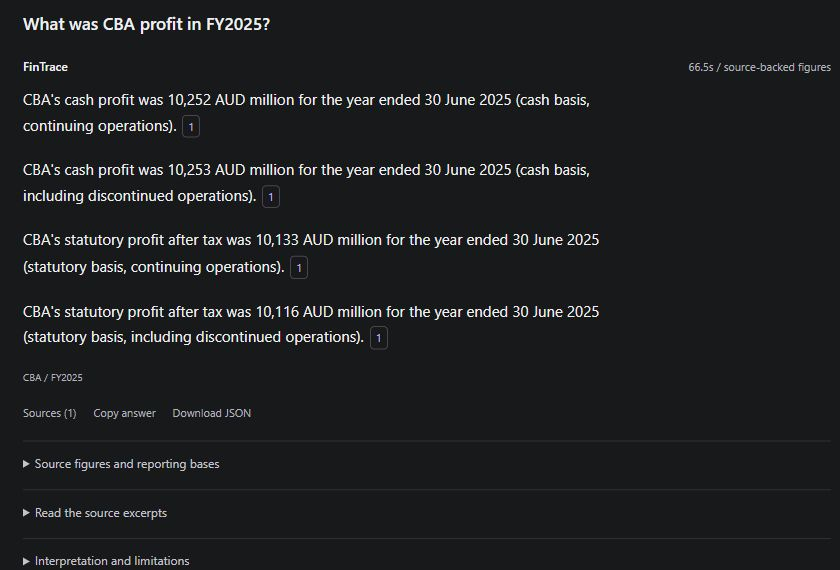
\includegraphics[width=0.98\linewidth]{frontend_profit.png}
\caption[Frontend: labelled profit alternatives]{Live interface response to ``What was CBA profit in FY2025?'' Four figures linked to source cells distinguish cash/statutory basis and continuing/total operations. The numbered references identify CBA's FY2025 Profit Announcement, PDF page 18~\cite{fintraceCBA2025}.}
\label{fig:frontend_profit}
\end{figure}

\begin{figure}[!htbp]
\centering
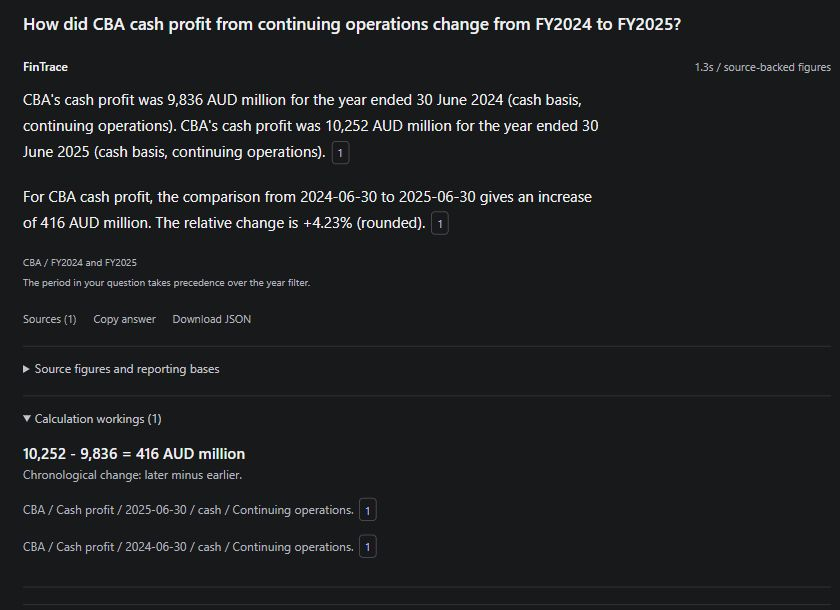
\includegraphics[width=0.98\linewidth]{frontend_comparison.png}
\caption[Frontend: comparison and calculation workings]{Live interface comparison of CBA continuing cash profit from FY2024 to FY2025. The expanded workings show AUD~10,252 million minus AUD~9,836 million, giving AUD~416 million; the answer reports approximately 4.23\% relative growth. Operand references lead to PDF page 18 of the FY2025 report. Screenshots are illustrative runs, not timing guarantees.}
\label{fig:frontend_comparison}
\end{figure}

The prototype runs locally for a single user. Its evidence, models and indexes require installation beyond cloning the repository. Model startup and competition for GPU resources can affect response time. Checks of interface state and server behaviour were recorded separately from financial answer assessment. Formal accessibility, multi-user load and analyst usability studies remain future work.

% AI-assisted shared draft prepared at Ayushi's request on 25 October 2026.
% Assigned reviewer: Janhavi Maheshwar Ghate. Verify packets and scoring with Hashini.
\subsection{Evaluation design and scoring criteria}
\label{subsec:evaluation_design}

Evaluation distinguished finding relevant evidence from producing a correct and complete answer. A response may contain a valid number yet use the wrong financial basis, omit a requested part or cite an unrelated page. We therefore assessed retrieval, financial correctness, completeness, citation support, appropriate refusals and response time separately~\cite{fintraceEval2026}.

Questions covered lookups, comparisons across years within a bank, calculations, definitions, management explanations and ambiguous wording. Boundary cases tested unavailable years, future outcomes, other companies, live prices and personal investment advice. Reference answers record the document, page, reporting period, unit, financial basis and business scope. Assessment also considers whether the requested information is available within the prototype's searchable or checked evidence.

Responses to answerable questions are classified as complete, partial, incorrect or unnecessarily declined. An appropriate refusal concerns unavailable information or a clearly stated scope boundary. Declining an answerable request remains a coverage or effectiveness limitation even when it avoids fabrication. Runtime errors are recorded separately. Correctness requires the right financial context; completeness requires every requested part, including both comparison values and the calculation when a change is requested.

Hit@5 measures whether relevant evidence appears among the first five retrieval results. Mean reciprocal rank rewards placing relevant evidence earlier. nDCG@5 evaluates the order of the first five results relative to relevance judgments. These retrieval measures require saved rankings and relevance labels; they cannot be inferred from final citations. Numerical matching can also consider rows outside the first five results. Citation checks instead establish whether the cited page supports a claim. Arithmetic checks inspect operands, formula, units and rounding, distinguishing percentage points from relative percentage growth.

Development tests guided fixes, while regression tests checked previously observed behaviour. Separate AI-assisted assessments used questions held outside the runtime repository, not an external human panel. Because the archived question file names both issuer PDFs and the development metric catalogue as references, separate authorship does not establish an entirely unseen assessment based only on the reports. Once questions informed a fix, they became development evidence. Software test counts and successful HTTP responses are not financial answer accuracy. Each result is therefore reported with its software version and sample size, separating appropriate refusals from missed answerable questions.

% AI-assisted shared draft prepared at Ayushi's request on 25 October 2026.
% Assigned reviewer: Hashini Santhanakrishnan. Confirm original runs with Janhavi.
\subsection{Evaluation procedure and validity safeguards}
\label{subsec:evaluation_procedure}

Before assessment, the procedure records the software version, model configuration and evidence files. Integrity checks compare the application and source files against a recorded list of checksums before and after testing. This establishes whether the system changed during the assessment, rather than whether its answers are financially correct~\cite{fintraceEval2026}.

Questions and expected answers remain separate from the runtime evidence. The evaluation script uses \texttt{serve\_fintrace\_demo.build\_backend()} so that it tests the configured application rather than generic defaults. Every first response is preserved, including errors and fallbacks, without retrying until a favourable answer appears. Response time is recorded separately from correctness.

Assessment examines the complete response, including displayed text, structured claims, calculations, quotations and limitations. This avoids an earlier evaluation adapter error that overlooked calculations stored outside the prose. Claims are checked against cited pages for the correct row, year, unit, financial basis, business scope and report version. Equivalent units and reasonable rounding are acceptable; substituting a neighbouring financial measure is not. An explanation that gives a correct figure without the requested reasons is incomplete.

Disagreements are investigated against the source before changing an answer or reference key. Original expectations and failed responses are retained alongside corrections. When an earlier year's figure comes from a later report's comparative column, that publication is identified. A difference from the original report does not by itself establish a formal restatement. Comparisons use compatible columns when calculating changes~\cite{fintraceCandidate2026}.

The main validity limits are small, deliberately selected question sets, AI-assisted judgments and changes in coverage during development. No independent human panel or controlled analyst study was conducted. Questions used for tuning cannot establish performance on unseen requests. Responses and timing may also vary between runs. Earlier results therefore apply to the versions tested, while the frontend screenshots illustrate functionality rather than provide a fresh accuracy estimate.


% AI-assisted shared draft prepared at Ayushi's request on 25 October 2026.
% Assigned reviewers: Janhavi (CBA) and Hashini (NAB). Verify original packets before approval.
% All counts retain historical candidates; no new model assessment was run for this edit.
\section{Findings}
\label{sec:Findings}

\subsection{What the recorded evaluations establish}
The results support a bounded reliability argument, not universal accuracy. Table~\ref{tab:evaluation_checkpoints} reconciles the historical review of 24 first responses from candidate \texttt{aa7fef9}. The public packet retains the original responses, questions and AI-assisted review~\cite{fintraceReleaseReview2026}. This report describes later implementation checkpoint \texttt{449c4ba}, not a newly assessed candidate with the same score.

\begin{table}[htbp]
\centering
\small
\caption{Historical 24-response review: exact named categories, not current accuracy.}
\label{tab:evaluation_checkpoints}
\renewcommand{\arraystretch}{1.15}
\begin{tabular}{p{0.48\linewidth}p{0.12\linewidth}p{0.29\linewidth}}
\hline
\raggedright\textbf{Recorded category} & \raggedright\textbf{Count / 24} & \raggedright\textbf{Question IDs} \tabularnewline
\hline
\raggedright Explicitly listed as correct and sufficiently complete & 12 & \raggedright D01--04, D08--12, D14, D19, D23 \tabularnewline
\raggedright Partial or limited & 4 & \raggedright D05, D07, D13, D15 \tabularnewline
\raggedright Over-refusal of an answerable item & 1 & D06 \tabularnewline
\raggedright Appropriate non-answer within declared scope & 6 & \raggedright D16--18, D21--22, D24 \tabularnewline
\raggedright Correct vintage example; completeness not categorised & 1 & D20 \tabularnewline
\hline
\textbf{Total} & \textbf{24} & D01--D24 \tabularnewline
\hline
\end{tabular}
\end{table}

The review recorded zero serious financial errors, misleading citations or runtime errors; these are separate checks, not additional outcome categories. D20 was discussed but not assigned a completeness category, so no exhaustive accuracy percentage is inferred. These historical judgments also predate the later expansion of generic-profit alternatives. Reference-key corrections and AI-assisted assessment limit the result's independence.

Development evidence is separate: 584 Python tests, ten frontend tests and 232 supported numerical wording checks passed. Another 24-response development run recorded seven unable-to-verify statuses (29.2\%: six boundary cases and one answerable refusal) and five partial statuses~\cite{fintraceCandidate2026}. Statuses and software checks are not financial correctness scores and are not pooled with Table~\ref{tab:evaluation_checkpoints}.

\subsection{Preliminary retrieval baseline}
The preliminary Walert exercise rebuilt BM25 search over 120 FAQ passages. Across 96 answerable questions, it achieved Hit@5 of 80.21\%, MRR of 0.6408 and nDCG@5 of 0.4190. Hit@5 was 82.14\% for 84 known/paraphrased questions and 66.67\% for twelve inferred questions. This wording gap helped motivate testing indirect requests rather than only exact metric names. Supplied Walert generation outputs were rescored, not regenerated; the full Falcon-7B pipeline was not reproduced~\cite{fintraceWalert2026}. These results concern a different corpus and task, so they are not a financial-answer baseline that FinTrace has beaten. A matched end-to-end ablation of the latest financial candidate remains a limitation.

\subsection{CBA: context, calculation and source checking}
CBA cases show why correctness and completeness need separate treatment. A general profit question initially returned cash and statutory alternatives, but later review identified four relevant FY2025 variants: continuing cash profit of AUD~10,252 million, total cash profit of AUD~10,253 million, continuing statutory profit of AUD~10,133 million and total statutory profit of AUD~10,116 million~\cite{fintraceCBA2025}. Totals include discontinued operations; they are not discontinued-only results. The later source-bound update is implementation evidence, not a result from the earlier 24-question assessment.

The historical release review accepted the continuing cash-profit comparison: AUD~9,836 million to AUD~10,252 million gives AUD~416 million, approximately 4.2\%. It also accepted the distinction between the largest investment-spending category, productivity and growth, and the largest increase, infrastructure and branch refurbishment. However, the investment response was verbose and included FY2023 context outside the requested window. Correct evidence did not automatically produce a concise answer.

A customer-deposits disagreement exposed a reference-key problem. The initial expectation used AUD~834,259 million, while the FY2025 report's FY2024 comparative column showed AUD~851,682 million. With FY2025 deposits of AUD~908,812 million, the compatible change is AUD~57,130 million, about 6.71\%. The original key was preserved and source headers were inspected rather than forcing a match~\cite{fintraceCandidate2026}. Evaluation assumptions required checking as carefully as system outputs.

\subsection{NAB: distinctions and incomplete explanations}
The historical review found labelled cash and statutory alternatives and correct supported calculations. A NIM movement of 0.03 percentage points was not presented as 3\% relative growth. Report-version disclosure also distinguished original FY2024 net operating income of AUD~20,250 million from the FY2025 report's comparative value of AUD~20,236 million, without automatically calling it a restatement~\cite{fintraceReleaseReview2026}.

Several responses remained incomplete. A question about why operating expenses rose returned figures and change without management's drivers. A capital-strength question retrieved CET1 commentary but omitted the headline movement from 12.35\% to 11.70\%. Cost-to-income was refused despite being available in the report. These are coverage or effectiveness failures, not proof that the information was absent. Later checked annual-report table paths widened coverage, but exposed follow-up questions cannot establish fresh generalisation performance~\cite{fintraceCoverage2026}.

\subsection{Answerability, latency and project questions}
In the 24-question historical review, six cases concerning cross-bank comparison, prediction, an excluded year, another bank, personal advice and live price received appropriate non-answers under the declared boundaries. No runtime errors or model/excerpt fallbacks occurred. Most numerical answers were reported as sub-second, but one comparison took approximately 178 seconds and a further answer about 35 seconds. These observations demonstrate variable latency, not a response-time guarantee~\cite{fintraceReleaseReview2026}.

The project questions are therefore answered unevenly. FinTrace can locate and label supported figures and calculate compatible within-bank changes. Explanations and definitions are report-grounded but less consistently complete than checked numerical answers. Source links and explicit limits make verification possible, while the key-correction case demonstrates why evaluation assumptions also need scrutiny. Whether these functions reduce analyst effort remains unmeasured. No current bank-specific aggregate accuracy is claimed without a fully adjudicated, version-matched set.

% AI-assisted shared draft prepared at Ayushi's request on 25 October 2026.
% Assigned reviewer: Guruprasad Simimath. Verify benefit claims and link final visuals.
\section{Impact and Significance of Results}
\label{sec:Impact and Significance of Results}

\subsection{Value for the analyst's task}
FinTrace addresses a specific step in preparing a financial briefing: finding a result, understanding its context and checking the source before reuse. Its value is not replacing financial judgment. It brings evidence, labels and supported workings together so that an analyst has less to reconstruct from a short, unsupported answer.

A user asking about profit may not know to specify cash or statutory basis and continuing or total operations. Showing available labelled alternatives reveals that choice rather than silently making it. Similarly, a within-bank comparison is more useful when its original values, formula and report version can be inspected. These functions are demonstrated in a working interface, not merely proposed.

One historical 24-question assessment recorded no serious financial errors or misleading citations, but some source-answerable questions remained incomplete or were refused~\cite{fintraceReleaseReview2026}. Avoiding wrong figures matters, yet excessive refusal also imposes work on the user. The target is useful coverage with visible uncertainty, not safety measured only by how few questions receive answers.

\subsection{Expected benefits and responsible use}
Less manual searching, easier checking and fewer unnoticed reporting-basis mistakes are plausible benefits, not established user-study findings. The project does not claim a percentage reduction in analyst time, financial losses or business risk. A suitable next study would compare manual report search with FinTrace on identical briefing tasks, measuring completion time, answer quality and verification effort.

Human review remains necessary before sign-off. Public reports may omit information; retrieval may miss it; relevant quotations may still fail to answer the question. Source vintage, entity boundaries and definitions must remain visible even when they make an answer longer. Historical spending does not establish future performance or investment suitability.

Local inference avoids sending questions to a hosted generation service in the configured demo, but does not certify enterprise security. The prototype has no production access-control model, formal security assessment or multi-user capacity validation. Nor has a formal accessibility audit been completed. These are deployment requirements, not demonstrated features.

\subsection{Priorities beyond the demonstration}
The first priority is analyst feedback on incomplete explanations, coverage gaps and the evidence display. Improvements should be assessed on fresh questions after the candidate is fixed, with exposed cases retained as regressions. Latency also needs measurement on an uncontended system before setting operational expectations.

Broader deployment requires reliable installation, monitored source updates, access controls and usability and accessibility checks. Expansion beyond banking requires new terminology and validated accounting relationships, not simply more PDFs. Keeping these priorities separate from demonstrated functionality avoids presenting a bounded source-checking assistant as general financial analysis.

% Report section owner: Ayushi Negi.
% AI-assisted working draft. Confirm completed contributions and mentoring/board evidence with the team.
% The allocation below is not verified authorship of every implementation module.
\section{Project Management}
\label{sec:Project Management}

\subsection{Organisation and responsibilities}
Our six-member group organised the project around data, retrieval, answer production, the user workflow, evaluation and integration. Ayushi led coordination and reviewed the pipeline from source selection through to final answers, bringing gaps back into development discussions. Table~\ref{tab:report_responsibilities} sets out the agreed workstreams and writing responsibilities. These allocations describe who reviews and explains each area; completed contributions are recorded separately in the contribution sheet.

\begin{table}[htbp]
\centering
\small
\caption{Team workstreams and final-report responsibilities.}
\label{tab:report_responsibilities}
\begin{tabular}{p{0.27\textwidth}p{0.65\textwidth}}
\toprule
Member & Responsibility \\
\midrule
Ayushi Negi & Coordination, development and evaluation review, extraction, problem definition, project management and final integration; screenshots and architecture. \\
Yash Keswani & Data scope and answer-generation workstream; document source selection, answer paths and model configuration. \\
Shriram Varadarajan & Retrieval workstream; document chunking, indexing, search decisions and evidence handoff. \\
Guruprasad Simimath & Frontend workstream; explain the user workflow and supplied visuals, business impact, limitations and future improvements. \\
Janhavi Maheshwar Ghate & CBA evaluation workstream; document evaluation design, scoring criteria and CBA findings. \\
Hashini Santhanakrishnan & NAB evaluation workstream; document procedure, validity safeguards and NAB findings. \\
\bottomrule
\end{tabular}
\end{table}

We shared progress through Trello and group chat. GitHub holds the implementation and preliminary Walert work, while Overleaf keeps the report and its editing history. The links are in Appendix~\ref{app:project_evidence}. Responsibilities changed from the Milestone~1 plan as the scope became clearer, so the final contribution record needs to reflect work actually completed, not just the original allocation.

\subsection{Planning, progress checks and review}
The early Walert exercise gave us a starting point for separating retrieval quality from the decision not to answer. We rebuilt a BM25 baseline and assessed supplied Walert outputs; we did not reproduce its full Falcon pipeline. The retained \href{https://github.com/AyushiNegi20/COSC2669-WIL-PROJECT/blob/report-submission-2026-10-25/walert_reproduction/RESULTS.md}{preliminary results} informed the later focus on both useful evidence and honest non-answers.

In Sprint~5, from 21 to 27~September, review focused on reliable figures, traceable sources and realistic questions. Trello and chat updates served as progress checks: an issue was raised, the relevant workstream was discussed and a fix was checked against the original question and earlier cases. This kept the work in small reviewable increments, although the records do not establish a formal daily stand-up schedule.

The \href{https://trello.com/c/akurkkvG}{Sprint~5 review card} links the technical chronology and records that broader reasoning and behavioural follow-up remained unfinished at the sprint boundary. That work carried into Sprint~6. Some cards were added retrospectively, so their sprint labels organise the work but do not prove when a meeting or code change happened. Dated commits and saved run files provide the technical timeline.

\subsection{Iteration through observed failures}
Our review loop was straightforward: ask a question, keep the response, inspect the cited page and work out where the answer went wrong. A miss could come from extraction, retrieval, interpretation, financial binding or presentation. We therefore checked the failing stage before deciding whether the next change should involve the evidence, routing, calculation or model.

The September extraction work compared table representations and added a logged correction for invisible brackets. Investment questions revealed another issue: the largest spending category is not necessarily the category with the largest annual increase. The checked investment path now keeps those answers separate. Reviewing comparisons also showed that an earlier-year figure taken from a later report needs its source version explained; it should not automatically be described as restated \cite{fintraceExtraction2026,fintraceCandidate2026}.

On 27~September, the coverage follow-up separated full-report reading from the checked numerical catalogue. It added NAB statement and reconciliation paths and repaired paragraphs split across PDF layout blocks. On 4--5~October, wording checks extended general-profit and EPS answers to the available labelled variants. The 13~October change distinguished a missing historical year from a request to predict future profit. Each change addressed an observed problem without implying that every report question was now covered \cite{fintraceCoverage2026,fintraceBroad2026,fintraceHistory2026}.

We retained failed responses and used exposed questions as regression cases. Separately authored assessment sets were kept outside the runtime index and tied to the candidate they tested. Once a result informed a fix, that set was no longer unseen. This prevented later versions from inheriting an earlier score without being assessed again.

\subsection{Mentor feedback, retrospective and delivery}
Mentor feedback on reasoning and behavioural questions pushed us beyond exact metric names. We tested wording such as where CBA was investing, then checked whether the evidence supported spending, lending or a ranking of categories. This made interpretation part of the review rather than assuming a relevant passage answered the question.

The retrospective recorded on the Sprint~5 review card identifies three lessons: retain failed responses, test realistic wording and freeze a stable demo rather than keep expanding it. The record was clarified on 2~October; it does not give an exact retrospective meeting date. A practical consequence was to prioritise bounded fixes and leave explanation, coverage and latency improvements visible in the \href{https://trello.com/c/6hV8pwiq}{post-demo backlog}. Reliable evidence handling mattered more than making every answer sound fluent.

Guruprasad, Yash, Shriram and Hashini contributed to the presentation slides, and Ayushi and Janhavi handled recording. Ayushi coordinated submission. The \href{https://trello.com/c/PA5l3gfM}{presentation-deck card} and \href{https://trello.com/c/aexWs4nM}{pre-recording checks} provide delivery evidence. Separate subsection files support report review without replacing one another's work. Ayushi prepared the architecture diagram, captured the frontend examples and integrated the AI-assisted section drafts and executive summary. The workstream table is a review allocation, not a claim that each member independently authored that implementation or draft.

The submission check reconciled the public repository with the report's implementation checkpoint and retained evaluation artifacts outside the runtime index. The final contribution sheet still requires the group's confirmation, and five personal reflections remain for their owners. A working demo does not establish completed individual contributions; these remaining confirmations cannot be inferred from code tests or assigned roles.

\clearpage
\begin{center}
    \noindent\textcolor{purple}{\emph{-- Content below this line does not count for the page/word limit. --}}
\end{center}
I certify that the submission of this assignment is incomplete without the submission of the completed \textbf{Condition 3 Bounded Process AI Declaration Form} (templates available in the specification of the assignment on Canvas).
\begin{acks}
We acknowledge the Wurundjeri people of the Kulin Nation as the Traditional Owners of the land on which RMIT's Melbourne City campus stands. We pay our respects to Elders past and present. We thank our mentor Syeda Khan and the teaching team for feedback on scope, reasoning questions and evidence-based evaluation. We also acknowledge the maintainers of Walert and the open source tools used in the prototype. We thank CBA and NAB for making the reports publicly available.


We acknowledge substantive assistance from ChatGPT/Codex and Claude with implementation, evaluation, report drafting and reflection drafts. The separately submitted Condition~3 Bounded Process AI Declaration provides the full account; Appendix~\ref{app:ai_process} gives an editing example.
\end{acks}
\bibliographystyle{ACM-Reference-Format}
\bibliography{99_references,FINTRACE_REFERENCE_ADDITIONS}
\appendix
% Coordinator: Ayushi Negi. Each member must write their own reflection.
\section{Project Evidence and Individual Reflections}
\label{app:project_evidence}

\subsection{Repositories, version records and coordination}
\label{app:implementation_versions}
The group submission repository is \href{https://github.com/AyushiNegi20/COSC2669-WIL-PROJECT}{COSC2669-WIL-PROJECT}. It contains the imported FinTrace application under \texttt{fintrace/}, the preliminary Walert reproduction and Milestone~1 records. Its \href{https://github.com/AyushiNegi20/COSC2669-WIL-PROJECT/blob/main/fintrace/docs/WIL_MIGRATION.md}{migration record} identifies the imported release and verification scope.

\textbf{Final implementation.} The report's implementation reference is the public WIL repository snapshot tagged \texttt{report-submission-2026-10-25}, corresponding to WIL commit \texttt{fab4ca9}. Its FinTrace application matches the recorded backend version \texttt{449c4ba}. The \href{https://github.com/AyushiNegi20/COSC2669-WIL-PROJECT/blob/report-submission-2026-10-25/report/IMPLEMENTATION_CHECKPOINT.md}{version record} explains the imported implementation and setup paths. These identifiers locate the code described in the report; they are not quality scores.

\textbf{Evaluated version.} The 24-question financial assessment in Section~\ref{sec:Findings} used the earlier backend version \texttt{aa7fef9}, with first responses retained in the \href{https://github.com/AyushiNegi20/COSC2669-WIL-PROJECT/tree/report-submission-2026-10-25/report/evidence/historical-release-20260926T233529Z}{assessment archive}. Subsequent fixes were checked through development and regression testing, but the earlier assessment is not presented as a fresh evaluation of the final implementation. The necessary implementation and evaluation evidence is available in the public WIL repository without access to the private development repository.

Coordination records are on the \href{https://trello.com/b/TlRdAYBm/cosc2669-wil-project}{WIL Project~9 Trello board}. The report is written in the \href{https://www.overleaf.com/project/6a825099db573616c529838b}{shared Overleaf project}, retaining version history. Current card status shows the state of a task; commits and run records establish the content and timing of technical changes.

\subsection{Failure analysis and evaluation provenance}
The \href{https://github.com/AyushiNegi20/COSC2669-WIL-PROJECT/blob/report-submission-2026-10-25/fintrace/docs/BANKING_PDF_EXTRACTION.md}{extraction comparison} showed why finding the digits was not enough. On the development sample, tools could recover a value in page text but fail to preserve its row relationship. This led to structure-aware extraction and separate checks of source characters and financial context. Because the sample also informed the fixes, it cannot establish accuracy on unseen pages.

The \href{https://github.com/AyushiNegi20/COSC2669-WIL-PROJECT/blob/report-submission-2026-10-25/fintrace/reports/coverage/REVIEW.md}{coverage review} challenged another assumption: a missing answer did not mean the PDF was missing. All six reports already had extractable text. Gaps also came from restrictive numerical scope, routing and paragraphs split across layout blocks. The response was to improve those stages while keeping calculations limited to checked values, rather than treating every extracted table as reliable.

A further lesson came from the expected answer for CBA customer deposits. The expectation used AUD~834,259 million for FY2024, while the FY2025 report's comparative column showed AUD~851,682 million. Comparing that column with FY2025 deposits of AUD~908,812 million gives a change of AUD~57,130 million, about 6.71\%. The \href{https://github.com/AyushiNegi20/COSC2669-WIL-PROJECT/blob/report-submission-2026-10-25/fintrace/reports/coverage/RELEASE_CANDIDATE.md}{source-based review} preserved the original expectation and explained the reporting-version difference. The lesson was to check the key as well as the system: a disagreement should be resolved from the source, not by changing the output until it matches a number.

The \href{https://github.com/AyushiNegi20/COSC2669-WIL-PROJECT/tree/report-submission-2026-10-25/report/evidence/historical-release-20260926T233529Z}{historical assessment packet} preserves 24 first responses, original expectations, the companion review and file hashes. Its reconciliation names all question IDs and explicitly leaves D20 outside a completeness category rather than inventing a score. The original expectations include the deposits-key error and an unsupported restatement label; these are retained with explanatory notes, not silently corrected. The question file also names the development metric catalogue as reference material. The assessment is therefore not presented as entirely unseen or based only on the source reports.

\subsection{Runtime settings and reproducibility}
\label{app:runtime_details}
Numerical and prose responses use the recorded local application configuration rather than a hosted API. The generation model is Qwen3 8B, Q4\_K\_M, through Ollama. Its context setting is 16,384 tokens. Task-specific output caps are 900 tokens for drafts, 160 for passage selection, 220 for intent planning and 400 for support review. Sampling settings include temperature 0.7, top-p 0.8 and top-k 20. The 35-second timeout applies to each model call rather than the complete response. These settings describe the application rather than the model's maximum supported context.

Structured dense retrieval uses Qwen3-Embedding-0.6B with float32 CUDA inference and exact similarity over local NumPy vectors. Reciprocal rank fusion uses rank constant 60. Embedding inputs are checked against a configured 32,768-token ceiling; the subsequent structured evidence pack has a separate budget of about 2,048 tokens. Child and parent chunk ceilings are 2,400 and 10,000 UTF-8 bytes, with at most three table rows in a child. Bytes and tokens are not interchangeable.

Configuration, source checksums, model revisions and integrity records are retained in the public WIL copy. Financial evidence and model files are supplied through a setup process that checks them against recorded file hashes. They are not embedded in the report. The release manifest detects changes; it does not certify financial correctness. Source and regression checks do not replace assessment on new questions after the software version has been fixed.

\subsection{AI-assisted editing example}
\label{app:ai_process}
\textbf{Before:} The draft solution description said the system declined questions ``when the reports can't support an answer.''

\textbf{After:} The report distinguishes evidence retrieved or checked by the prototype from information that may exist elsewhere in the PDFs: ``When evidence is insufficient, the response describes the limitation rather than claiming the full report lacks an answer.''

\textbf{Annotation:} AI feedback identified that a retrieval miss does not establish absence from a report. The revised wording narrows the claim to the available evidence, consistent with the coverage failures we investigated. Selecting the bounded scope and accepting or rejecting revisions remain group decisions. AI also contributed substantive code, evaluation and report drafts; this wording example is not the full extent of its use. The repository's \href{https://github.com/AyushiNegi20/COSC2669-WIL-PROJECT/blob/report-submission-2026-10-25/report/AI_USE.md}{AI-use account} and accompanying Condition~3 declaration must be read together.

% Teammate reflections below are AI-assisted starting drafts based on assigned report sections.
% Each member must confirm completed work, personalise the account and approve it before submission.

\subsection{Ayushi Negi: Individual Reflection}
% AI-assisted reflection drafted earlier in this chat; inserted at Ayushi's request on 25 October 2026.
As project lead, I worked across development, evaluation and coordination. I reviewed the pipeline from source selection and PDF extraction through to chunking, retrieval, answer generation and the frontend. I also helped investigate failed answers, prepare the demonstration and organise the final report.

My biggest challenge was knowing when FinTrace was good enough. Each round of testing uncovered another gap. I sometimes felt that improving the system meant adding more features or trying a stronger model. Over time, I realised that a fluent answer could still be based on the wrong evidence. The important question was not simply whether the model sounded convincing, but whether it had answered the actual question with the right financial context.

The CBA profit example made this clear. Returning two correct figures could still be incomplete when the report contained four relevant variants. Similarly, making the full reports searchable improved coverage, but did not automatically make every table reliable for calculations. These experiences helped me distinguish retrieval, correctness and completeness instead of treating them as one measure of success.

I used AI tools to explore approaches and assist with implementation and evaluation. However, repeated suggestions also expanded the scope and created more back and forth. I learned to ask for evidence, preserve failed responses and judge changes against a fixed set of requirements.

Leading the project also showed me that taking on more work myself is not always the best way to coordinate a team. Next time, I would agree on smaller deliverables, clearer ownership and completion evidence earlier. I would also protect an unseen evaluation set and set release criteria sooner, so we could improve the system without continually moving the finish line.

\subsection{Yash Keswani: Individual Reflection}
My assigned report sections cover the source reports, PDF extraction and answer generation. These stages connect the financial documents to the final response, so their relationships matter as much as the tools used.

The extraction work highlights why a number must retain its year, unit and reporting basis to remain meaningful. The initial checks on selected pages and the later prose search across the full reports serve different purposes. Wider coverage helps find explanations, but it does not make every extracted table safe for calculations.

Another important distinction is between selecting evidence and writing an answer. A stronger model can produce clearer wording while still using the wrong evidence. The project therefore links values to source cells and uses Python for supported calculations, with Qwen helping select and explain passages. A model therefore needs to be assessed for reliability and response time rather than selected by size alone.

In a future project, I would define the extraction checks and record model settings earlier.

\subsection{Shriram Varadarajan: Individual Reflection}
My assigned report section focuses on chunking, indexing and retrieval. The central challenge is finding evidence that answers the actual question while retaining its financial meaning.

The pipeline demonstrates the importance of preserving table structure when creating chunks. A value needs its row label, year column, unit and reporting basis. Small searchable chunks can help locate a relevant item, while their parent context helps explain what that item means. Metadata identifying the company, period and source page also reduces the risk of using a plausible figure from the wrong context.

Structured evidence and prose from the full reports follow different search paths. This makes it important to describe the implemented system accurately rather than call every search hybrid retrieval. It also shows that semantic search needs to be evaluated on relevant questions rather than assumed to improve retrieval.

For a future iteration, I would compare retrieval methods on the same set of indirect questions and retain their ranked results.

\subsection{Guruprasad Simimath: Individual Reflection}
My assigned sections cover the frontend workflow, business impact and practical limitations. These areas connect the technical pipeline to the analyst's decision about whether an answer is useful enough to investigate or reuse.

The profit example illustrates why interface design is more than appearance. Four relevant figures need clear labels for cash or statutory basis and continuing or total operations. A short answer without those distinctions could be easy to read but incomplete. Source links and calculation workings give the user a way to inspect the answer instead of relying only on confident wording.

The business impact discussion requires a distinction between demonstrated functions and expected benefits. The prototype demonstrates source checking and supported calculations, but that does not prove measured time savings or lower analyst error rates. Those benefits would need a user study. Similarly, a local demo for a single user is not evidence of readiness for wider deployment.

In future work, I would involve intended users earlier and test whether they understand partial answers and evidence limits.

\subsection{Janhavi Maheshwar Ghate: Individual Reflection}
My assigned report responsibility covers the evaluation framework and CBA findings. The main issue is deciding what a successful answer means. Correct figures, complete answers, relevant sources and appropriate refusals are related, but they are not interchangeable.

The CBA cases make this distinction concrete. Two correctly labelled profit figures can still leave out relevant alternatives. The disagreement about customer deposits also shows why the answer key needs checking: a difference between report versions can make an expected figure unsuitable for a particular comparison. The source headers and reporting period matter as much as the digits.

Another important reporting decision is keeping software tests separate from assessment of financial answers. Passing hundreds of regression checks does not establish universal accuracy. Historical results must retain their candidate version, denominator and limitations, including AI-assisted judgments. Once questions have guided fixes, they are regression material rather than an untouched assessment set.

Next time, I would agree the scoring categories and protect unseen questions earlier.

\subsection{Hashini Santhanakrishnan: Individual Reflection}
My assigned report sections cover NAB findings and evaluation validity. A central challenge is distinguishing an incorrect answer from an incomplete explanation, an unsupported request or a retrieval gap. Treating all of these as the same failure would hide useful information about the system.

The NAB examples highlight how easily financial context changes an answer. Cash earnings and statutory profit are different measures, while a change in net interest margin should be expressed in percentage points. A later report's comparative value may differ from the earlier publication, so the source version must be disclosed without automatically calling the difference a restatement.

The assessment procedure also needs to inspect the whole response. An earlier evaluation adapter overlooked calculations stored outside the prose, demonstrating that the evaluation tools also require checking. Preserving first responses, checking the configured backend and recording latency separately make the findings easier to audit. None of these steps makes AI-assisted scoring equivalent to independent human review.

For future work, I would use a shared scoring guide and record disagreements explicitly.

\end{document}
